\documentclass[12pt,titlepage]{article}

\usepackage{amsmath,amssymb}
\usepackage{hyperref}
\usepackage{pgfplots}
\usepackage{siunitx}
\usepackage{placeins}
\usepackage{url}

\title{The Stroop Effect \\ \vspace{10pt} \large{\it Udacity Deep Learning Nanodegree Statistics Project}}
\author{George Yu}
\date{\today}

\begin{document}

\maketitle

\section{Basic Information}
  \begin{itemize}
    \item {\bf Independent Variable}: the congruency of the words and the ink colors
    \item {\bf Dependent Variable}: the time for the participant to name the ink colors in a list of words
  \end{itemize}
  
  According to \cite{wiki:stroop-effect}, the participants will take longer to name the ink colors for the incongruent words, so the we should perform a one-tailed test on a sample. The null hypothesis is that for the population, there is no difference in both groups of words, and the alternative hypothesis is that the time taken for the incongruent group will be longer than the congruent group in the population, or,
  \begin{align*}
    &\mathbf{H_0}\hspace{-2pt}:\ \mu_\mathrm{i} - \mu_\mathrm{c} \leqslant 0 \\
    &\mathbf{H_a}\hspace{-2pt}:\ \mu_\mathrm{i} - \mu_\mathrm{c} > 0,
  \end{align*}
  where $\mu_\mathrm{i}$ is the population mean of the time for the incongruent words, and $\mu_\mathrm{c}$ is the population mean of the time for the congruent words.
  
  Since each participant will go through and record from each of the two conditions, so this experiment is a within-subject design, namely, it tests a sample of $n=24$ with two conditions. Therefore, a dependent samples $t$-test should be used. The reason for using a $t$-test rather than a $z$-test is that the we do not know the population parameters $\mu$ and $\sigma$.
  
  To conduct the $t$-test, we make the following assumptions:
  \begin{itemize}
    \item The population is approximately normally distributed
    \item The sample drawn from the population should be random
    \item The sample data can estimate population parameters
    \item The dependent variable (time to read the words) is continuous
    \item The pair-differences $\overline{x}_\mathrm{d}$ are independent of each other
  \end{itemize}


\section{Dataset}
  \autoref{fig:histogram} shows a visualization of the dataset. From this graph, we can see that the incongruent group are mainly distributed to the right of the congruent group. The congruent group is mainly distributed between 8.63 and 19.28, while the incongruent group is mainly distributed between 13.96 and 24.61.
  
  For the congruent group, the mean is $\overline{x}_\mathrm{c} \approx 14.05$ with a sample standard deviation of $s_\mathrm{c} \approx 3.56$, and for the incongruent group, we have $\overline{x}_\mathrm{i} \approx 22.02$ and $s_\mathrm{i} \approx 4.80$.
  
  \begin{figure}[h]
  \centering
    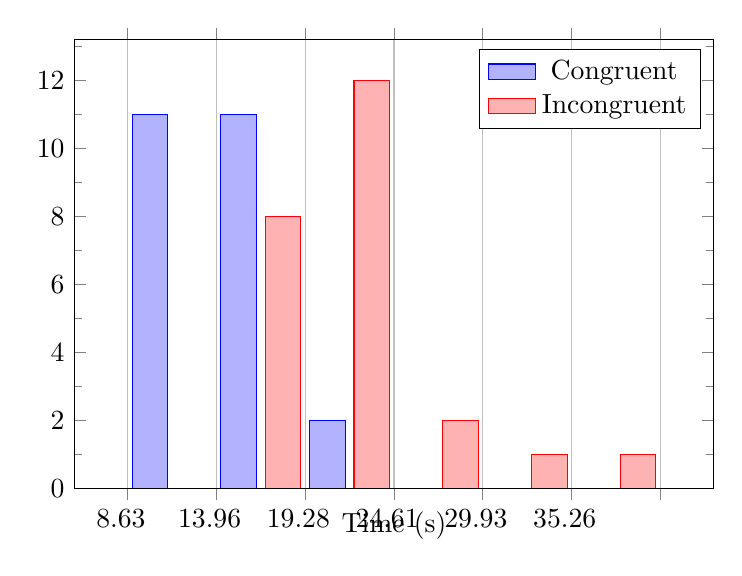
\begin{tikzpicture}
    \begin{axis}[
      width=0.8\textwidth,
      height=0.6\textwidth,
      x tick label style={xshift=-0.65cm},
      xlabel=Time (\si{s}),
      x label style={at={(axis description cs:0.5,-0.03)},anchor=north},
      enlarge y limits=upper,
      minor y tick num = 1,
      ybar interval=0.8,
      area style,
    ]
    \addplot+[ybar interval,mark=no] plot coordinates { (8.63, 11) (13.96, 11) (19.28, 2) (24.61, 0) (29.93, 0) (35.26, 0) (40.59, 0) };
    \addplot+[ybar interval,mark=no] plot coordinates { (8.63, 0) (13.96, 8) (19.28, 12) (24.61, 2) (29.93, 1) (35.26, 1) (40.59, 0) };
    \legend{Congruent,Incongruent}
    \end{axis}
    \end{tikzpicture}
    \caption{Data of }
    \label{fig:histogram}
  \end{figure}


\FloatBarrier
\section{Statistical Test}
  First subtract the incongruent group with the congruent group, we get a new distribution of differences with $\overline{x}_\mathrm{d} \approx 7.96$ and $s_\mathrm{d} \approx 4.86$.
  
  Using $\alpha = 0.05$, we obtain that our one-tailed $t$-critical value with $n=24$ (degrees of freedom $\nu = 23$), is $t^*=1.711$. Now, we can obtain the $t$-statistic,
  $$ t = \frac{\overline{x}_\mathrm{d} - \mu_0}{s_\mathrm{d}/\sqrt{n}}, $$
  where $\mu_0$ is the expected mean difference, which is $\mu_\mathrm{i} - \mu_\mathrm{c} = 0$, thus,
  $$ t = \frac{7.96}{4.86 / \sqrt{24}} \approx 8.02. $$
  
  We can see that $t$ is statistically significant, since $p < .0001$, in conclusion,
  $$ t(23) = 8.02,\ p < .0001,\ \textrm{one-tailed}. $$
  So, $\overline{x}_\mathrm{d}$ is significant at $p<0.05$, in other words, the difference in the two test groups are very unlikely due to chance, and since we are estimating the population parameter, we have $\mu_\mathrm{i} - \mu_\mathrm{c} > 0$, therefore we reject the null hypothesis. The result is what I expected.
  The $95\%$ confidence interval $CI$ is,
  $$ 95\%\ CI = (5.91, 10.01). $$


\section{Evaluation}
  Cohen's d is about 1.64, and the $r^2$ value is approximately $0.74$, which means that about 74\% of the variation in the time taken to name the ink colors can be explained by the congruency of the words and the ink colors. Other factors that might have influenced the time could be the carry-over effect, the order of the tests that the participants take will perhaps influence their results.
  
  We can conduct a similar experiment but using a between-subject design, where two independent samples are selected randomly, and one group will be reading the congruent words where the other group will be reading the incongruent words. This experiment can then eliminate the possible inaccuracies caused by the carry-over effect.


\medskip
 
\bibliographystyle{unsrt}
\bibliography{stroop}

\end{document}
